% =====================================================================
%  Selection push-down on the Sailors/Reserves plan, after [L14, s.22]
%  Compile:  pdflatex selection-pushdown.tex   (inside this folder)
%  Output:   selection-pushdown.pdf  -> 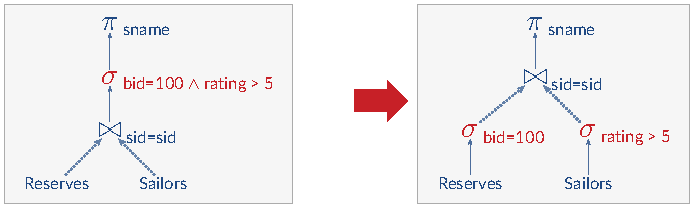
\includegraphics{selection-pushdown}
% =====================================================================
\makeatletter\def\input@path{{../../theme/}}\makeatother   % shared palette
\documentclass[tikz,border=2pt,11pt]{standalone}
\usepackage[T1]{fontenc}
\usepackage[defaultsans]{lato}
\renewcommand{\familydefault}{\sfdefault}
\usepackage{amsmath,amssymb}
\usepackage{vinuni-palette}
% Shared TikZ styles for the push-down figures (selection-pushdown.tex,
% projection-pushdown.tex), after the plan trees in [L14, s.22 and s.24].
% Not compiled on its own: \input by those files.
\usetikzlibrary{arrows.meta,shapes.arrows,fit,backgrounds}
\tikzset{
  op/.style   ={inner sep=0.6pt, text=vinuNavy},                       % operator symbol
  lab/.style  ={font=\scriptsize, anchor=west, inner sep=0.4pt},       % operator subscript
  rel/.style  ={font=\scriptsize, text=vinuNavy, inner sep=1pt},       % base relation
  un/.style   ={-{Stealth[length=1.2mm]}, vinuNavy!80},                % unary input
  bin/.style  ={-{Stealth[length=1.2mm]}, densely dotted, thick, vinuNavy!70},  % join input
  panel/.style={draw=vinuGray!70, fill=vinuLightGray!70, inner xsep=3mm, inner ysep=2mm},
  goes/.style ={single arrow, fill=vinuRed, draw=none, minimum height=9mm,
                minimum width=7mm, single arrow head extend=1.2mm},
}
% \opn[colour]{name}{(x,y)}{symbol}{subscript}: operator + subscript label
\newcommand{\opn}[5][vinuNavy]{%
  \node[op, text=#1] (#2) at #3 {\Large$#4$};
  \node[lab, text=#1] (#2l) at ([xshift=0.2mm, yshift=-1.2mm]#2.east) {#5};}
\newcommand{\hi}{vinuRed}   % colour of the operators that the rewrite changes


\begin{document}
\begin{tikzpicture}[x=1mm, y=1mm]
  % ---- before: one selection above the join -------------------------
  \begin{scope}[local bounding box=L]
    \opn{p}{(0,0)}{\pi}{sname}
    \opn[\hi]{s}{(0,-9)}{\sigma}{bid=100 $\wedge$ rating > 5}
    \opn{j}{(0,-18)}{\bowtie}{sid=sid}
    \node[rel] (r) at (-9,-27) {Reserves};
    \node[rel] (t) at ( 9,-27) {Sailors};
    \draw[un] (s) -- (p);  \draw[un] (j) -- (s);
    \draw[bin] (r) -- (j); \draw[bin] (t) -- (j);
  \end{scope}

  \node[goes] at (45,-13) {};

  % ---- after: each conjunct pushed onto its own input ----------------
  \begin{scope}[xshift=72mm, local bounding box=R]
    \opn{p}{(0,0)}{\pi}{sname}
    \opn{j}{(0,-9)}{\bowtie}{sid=sid}
    \opn[\hi]{s1}{(-11,-18)}{\sigma}{bid=100}
    \opn[\hi]{s2}{( 9,-18)}{\sigma}{rating > 5}
    \node[rel] (r) at (-11,-27) {Reserves};
    \node[rel] (t) at (  9,-27) {Sailors};
    \draw[un] (j) -- (p);
    \draw[bin] (s1) -- (j); \draw[bin] (s2) -- (j);
    \draw[un] (r) -- (s1);  \draw[un] (t) -- (s2);
  \end{scope}

  \begin{scope}[on background layer]
    \node[panel, fit=(L)] {};
    \node[panel, fit=(R)] {};
  \end{scope}
\end{tikzpicture}
\end{document}
